\chapter{Adaptatations in Animals}
\section{\textbf{Get Rolling}}
\textbf{Match the animals to the places which they are generally found.}\
\begin{enumerate}
    \item Camel - Desert
    \item Polar Bear - Polar and Mountain Regions
    \item Monkey - Forest
    \item Fish - River
\end{enumerate}
\section{\textcolor{red}{What to Know}}
The meaning of adaption and the ways in which different animals adapt themselves to their surroundings.
\section{\textbf{Learning Objectives}}
\begin{itemize}
    \item to classify different types of habitats
    \item to identify the breathing organs of different animals
    \item to compare the movements of different animals
    \item to analyse the behavioural adaptations of different animals
\end{itemize}
Different animals live in different places. They have some unique features that help them survive at those places. Let us learn more about them.
\section{\textcolor{red}{Habitats}}
The natural home or surroundings of an animal where it lives, grows, eats and reproduces its called its \textbf{habitat.}\\
\par
Habitats can be found all around us - forests, seas and oceans, lakes, ponds and rivers, polar and mountain regions, desert and grasslands. They can be on land or in water.\\
\par
Let us discuss some of the common habitats.
\subsection{\textcolor{orange}{Forest}}
A \textbf{forest} is a piece of land that has a large numbers of trees and plants growing in it. It receives moderate to heavy rainfall. Many types of birds, animals and insects live in a forest. There are forests were animals like lions, monkeys, deer, elephants, and squirrels live.
\begin{figure}
    \centering
    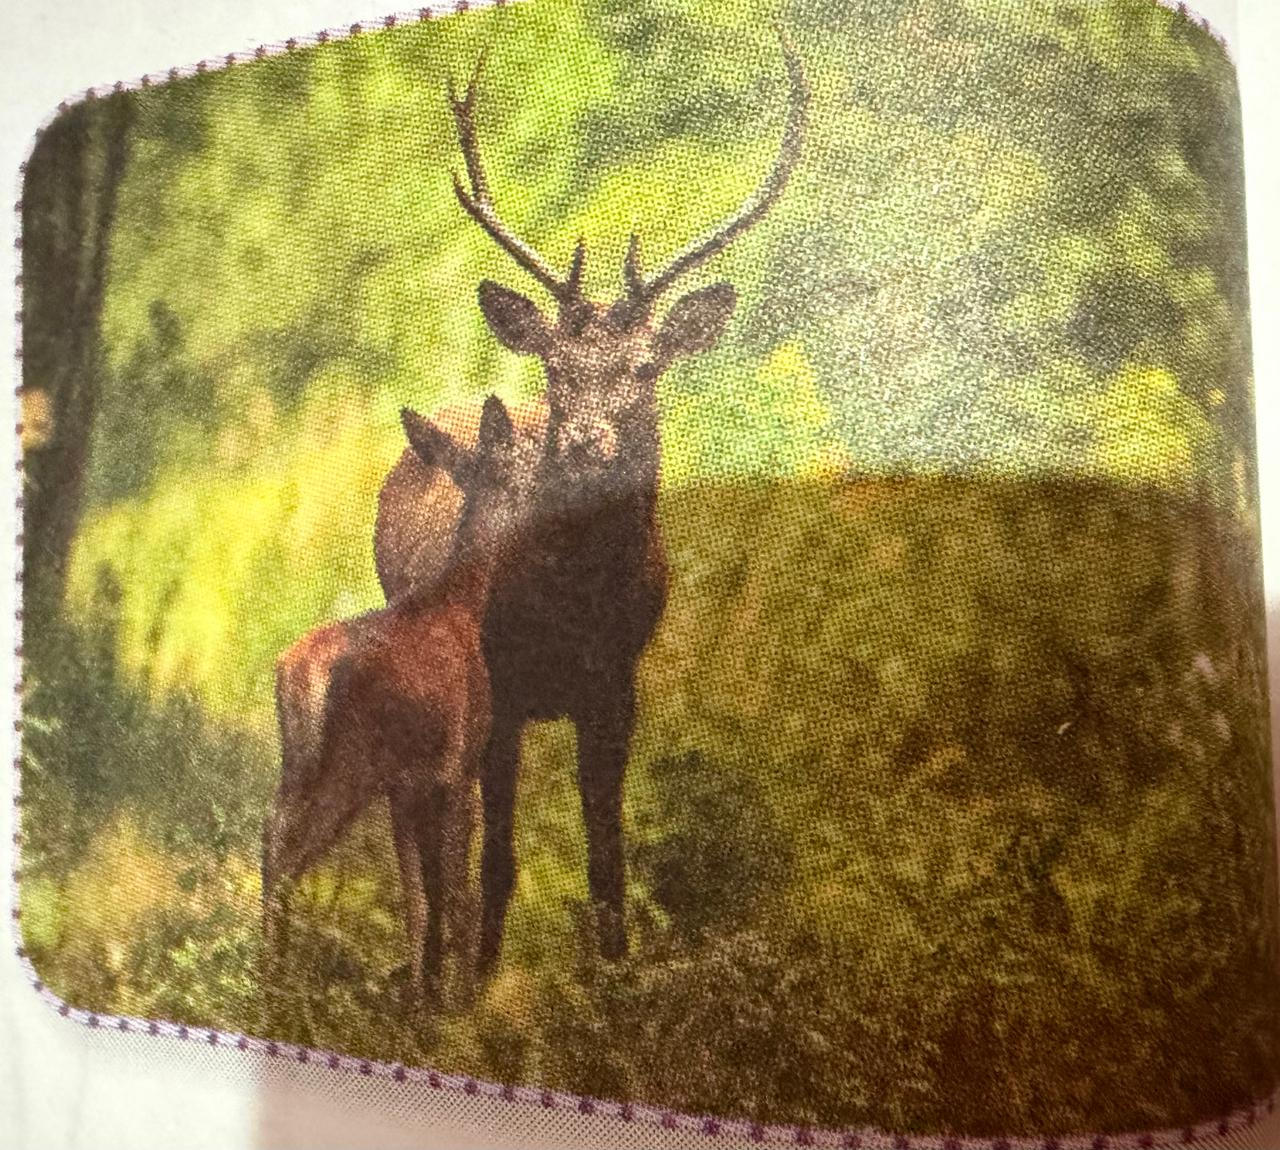
\includegraphics[width=0.5\linewidth]{../image/deer.jpeg}
    \caption{Caption}
    \label{fig:deer}
\end{figure}
\subsection{\textcolor{orange}{Desert}}
A \textbf{desert} is a dry, sandy and hot habitat. It receives very little rainfall.\\
\begin{figure}
    \centering
    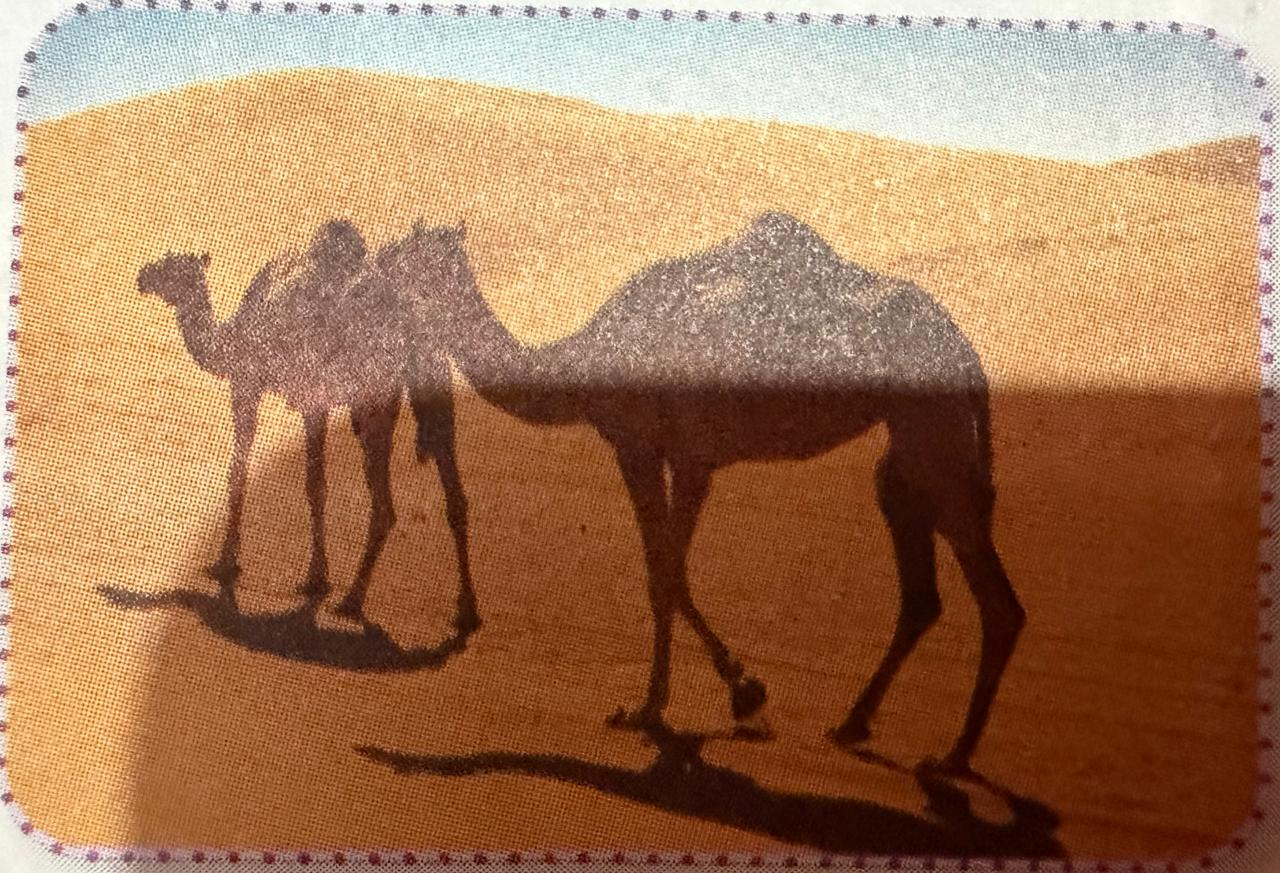
\includegraphics[width=0.5\linewidth]{../image/camel.jpeg}
    \caption{Caption}
    \label{fig:camel}
\end{figure}
\par
Animals such as snakes, scorpions, and camels live here.
\subsection{\textcolor{orange}{Polar and Mountain Regions}}
Polar and mountain regions are generally covered with snow, and they extremley cold throughout the year.\\
\par
Polar bears, seals and snow leopards are some animals found in these regions.
\begin{figure}
    \centering
    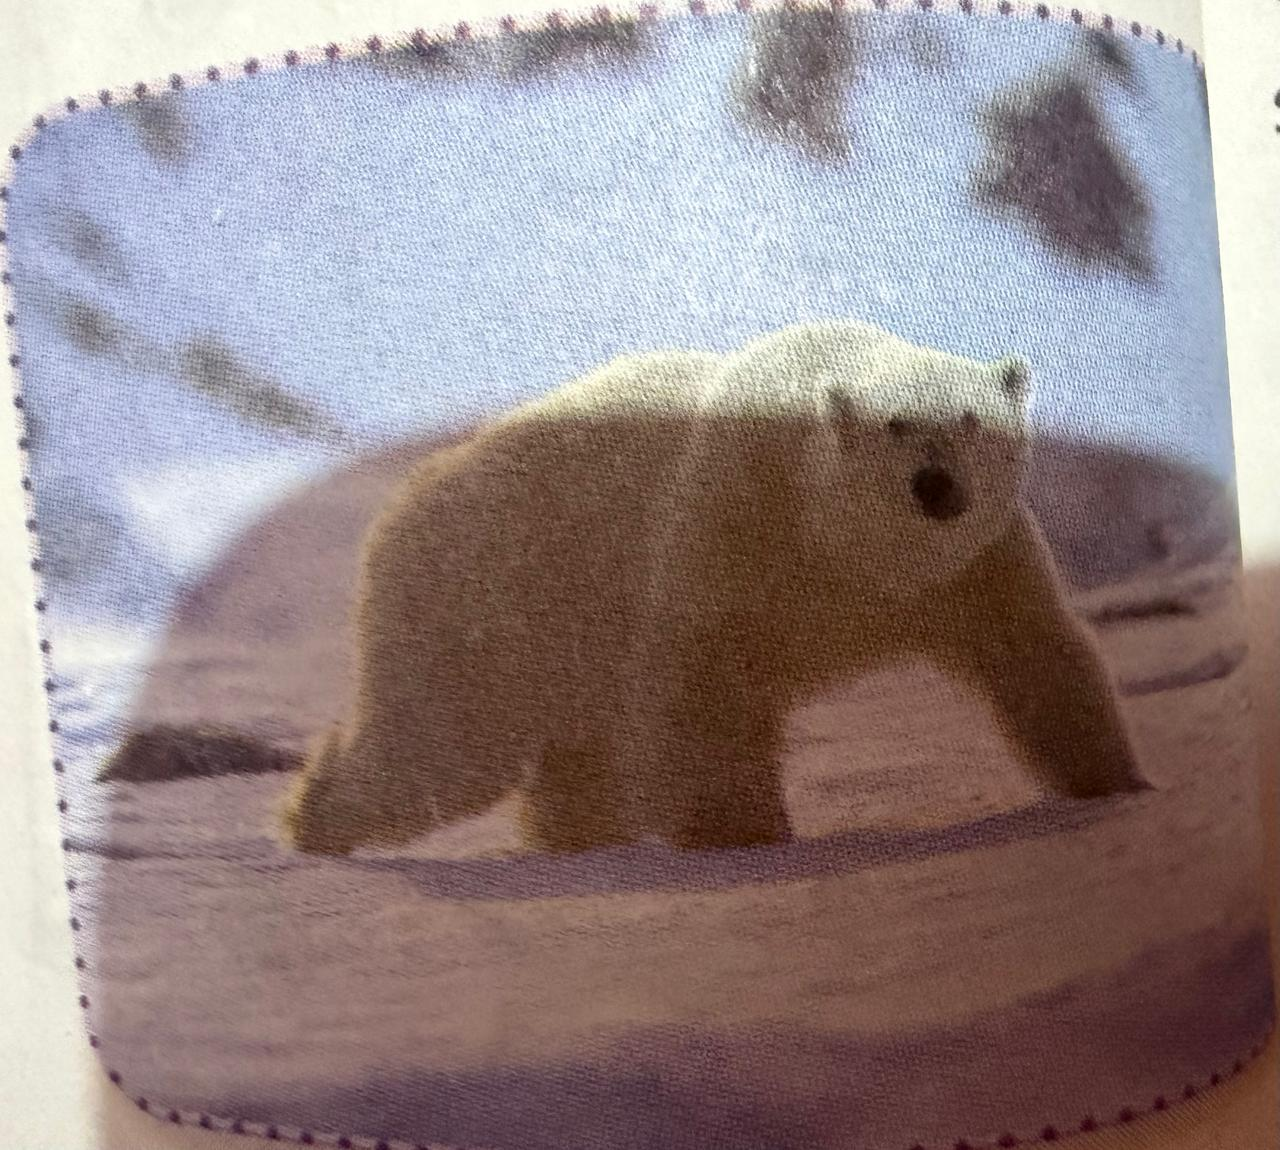
\includegraphics[width=0.5\linewidth]{../image/polar_bear.jpeg}
    \caption{Caption}
    \label{fig:polar-bear}
\end{figure}
\subsection{\textcolor{orange}{Lakes, Ponds and Rivers}}
Lakes, ponds and rivers are home to a variety of aquatic animals. Lakes, ponds and rivers are freshwater sources. The animals found here are different from the animals found in seas and oceans.\\
\begin{figure}
    \centering
    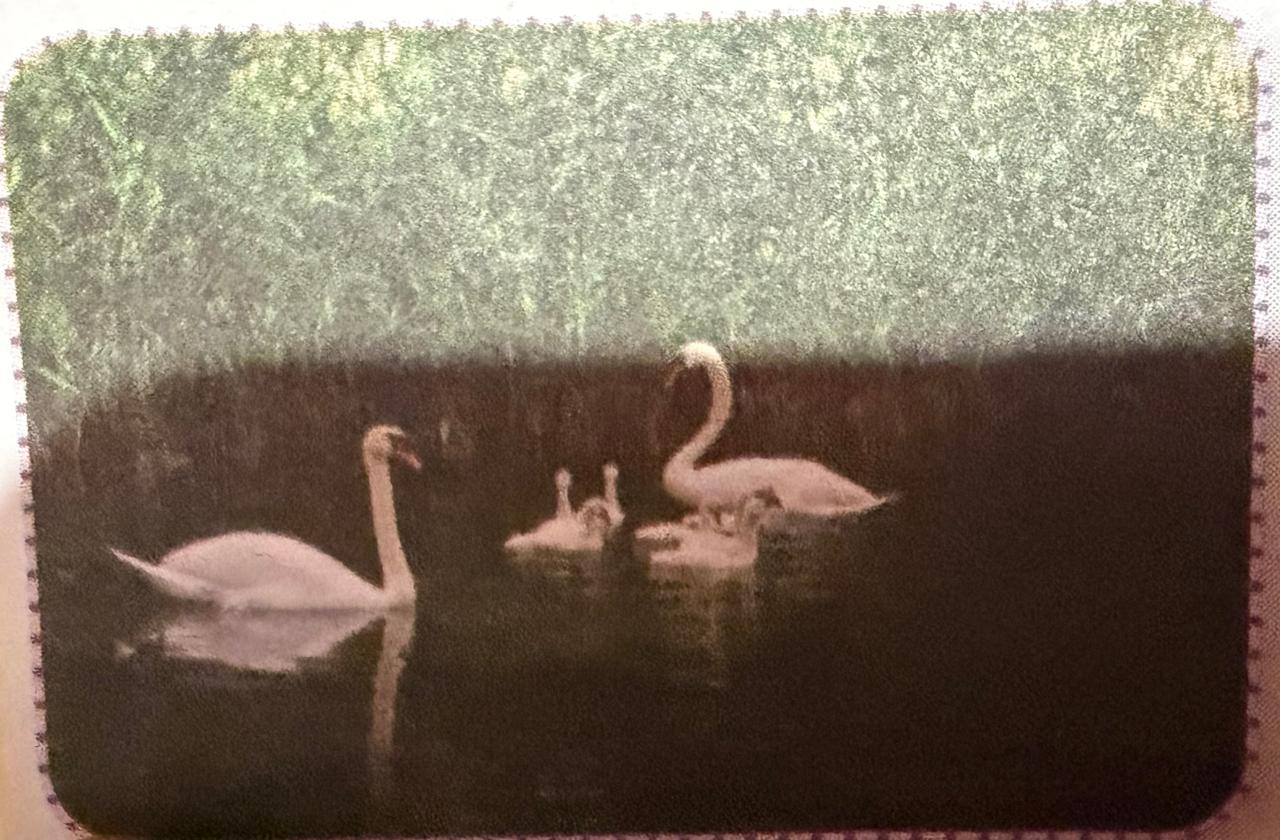
\includegraphics[width=0.5\linewidth]{../image/duck.jpeg}
    \caption{Caption}
    \label{fig:duck}
\end{figure}
\par
Example include frogs, fish, swans and ducks.
\subsection{\textcolor{orange}{Seas and Oceans}}
An \textbf{seas and oceans} is a vast habitat of a wide variety of marine life, including fish, crabs, sea turtles, dolphins and whales.\\
\par
Seas and oceans have salty water. Therefore, the animals that can live only in salty water live in this habitat.\\
\par\vspace{0.8in}
Based on their habitats, amimals have different body features and exhibit different behaviors that help in survive in their habitats.
\begin{figure}
    \centering
    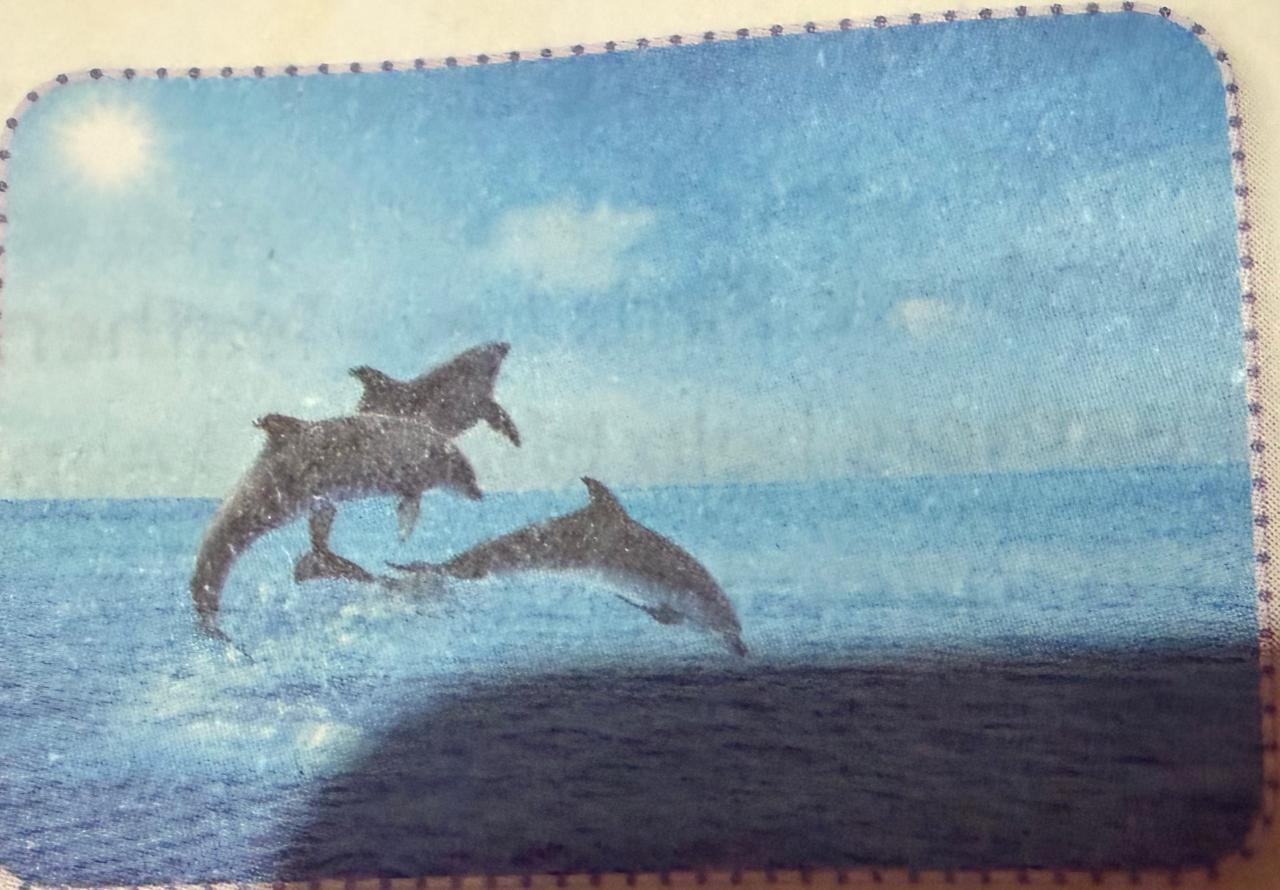
\includegraphics[width=0.5\linewidth]{../image/dolphin.jpeg}
    \caption{Caption}
    \label{fig:dolphin}
\end{figure}
\section{\textcolor{red}{Adaptations}}
\textbf{Adaptation} refers to the process by which organisms undergo changes in their physical structures and behaviours in the response to their environment. These changes are not sudden but occur gradually over long period.
\subsection{\textcolor{orange}{Adaptations in Physical Structures}}
Animals have different types of body coverings that help them survive in their environments.\\
\par
\textbf{Fur or Hair:} Many mammals, like dogs, cats and bears, have fur or hair covering their bodies. Fur helps to keep them warm in cold wheather. They also help them blend into their environment. Look at how polar bear is almost invisible in the snow. This is called camouflage. \textbf{Camouflage} is the ability of animals to blend into their surroundings to hide from predators or to \textcolor{red}{sneak} up on their prey.\\
\begin{figure}
    \centering
    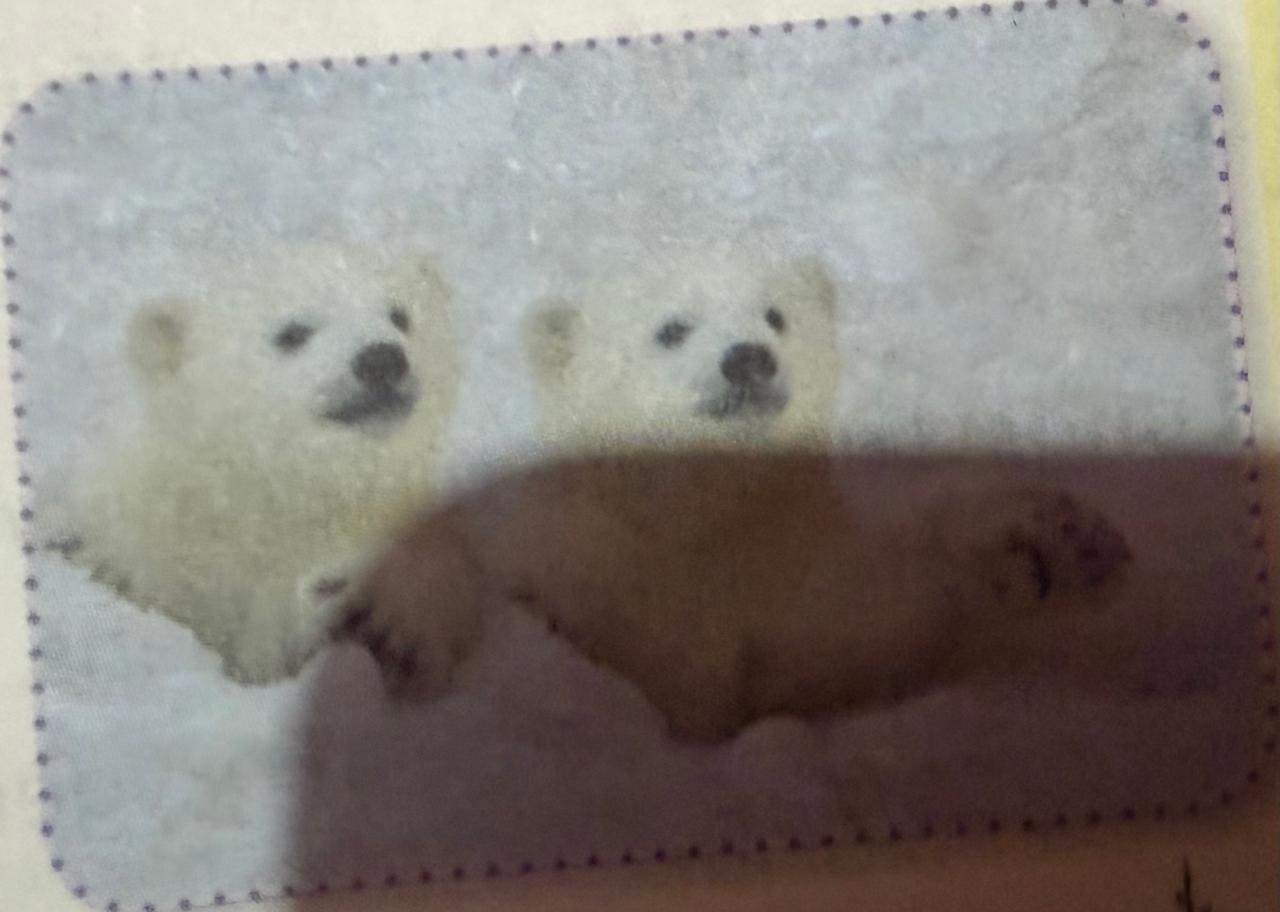
\includegraphics[width=0.5\linewidth]{../image/baby_polar_bear.jpeg}
    \caption{Caption}
    \label{fig:baby}
\end{figure}
\par
\textbf{Feathers:} Birds have feathers that cover their bodies. Feathers help birds fly, keep them warm and provide them waterproofing during rain.\\
\begin{figure}
    \centering
    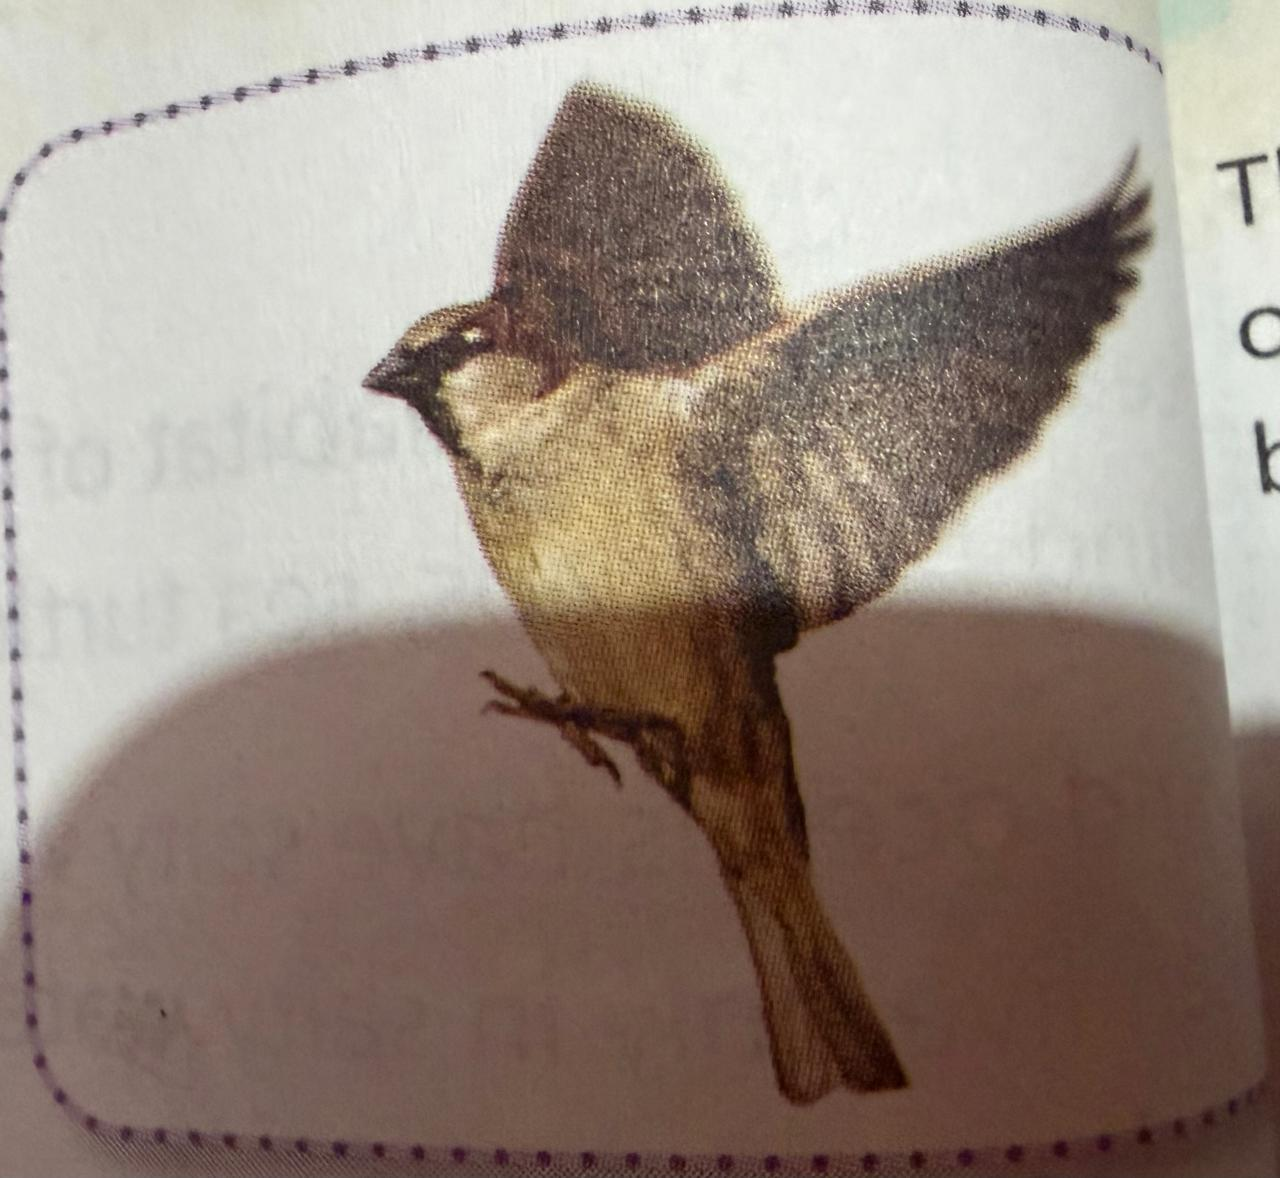
\includegraphics[width=0.5\linewidth]{../image/feather.jpeg}
    \caption{Caption}
    \label{fig:feather}
\end{figure}
\par
\textbf{Scales:} Fish and reptiles have scales. Scales provide protection and help in their movement. In fish, scales are flexible and allow smooth swimming, while in reptiles scales are rigid and act as a barrier against rough surfaces.\\
\begin{figure}
    \centering
    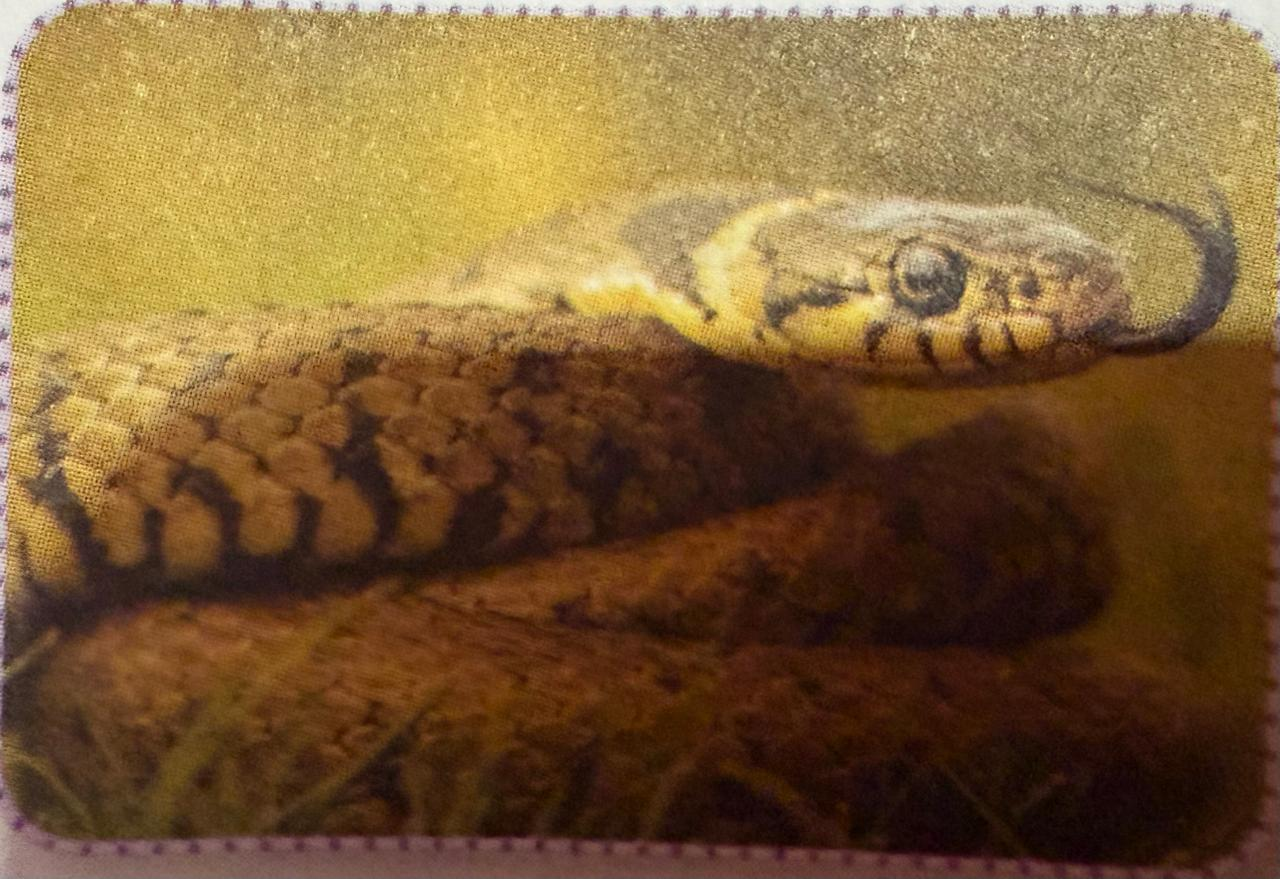
\includegraphics[width=0.5\linewidth]{../image/snake.jpeg}
    \caption{Caption}
    \label{fig:snake}
\end{figure}
\par
\textbf{Shells:} Some animals like turtles and snails have shells covering their bodies. Shells are hard and protect these animals from predators. They also provide a safe place to hide when needed. Shells are of different shapes and sizes in different animals.
\begin{figure}
    \centering
    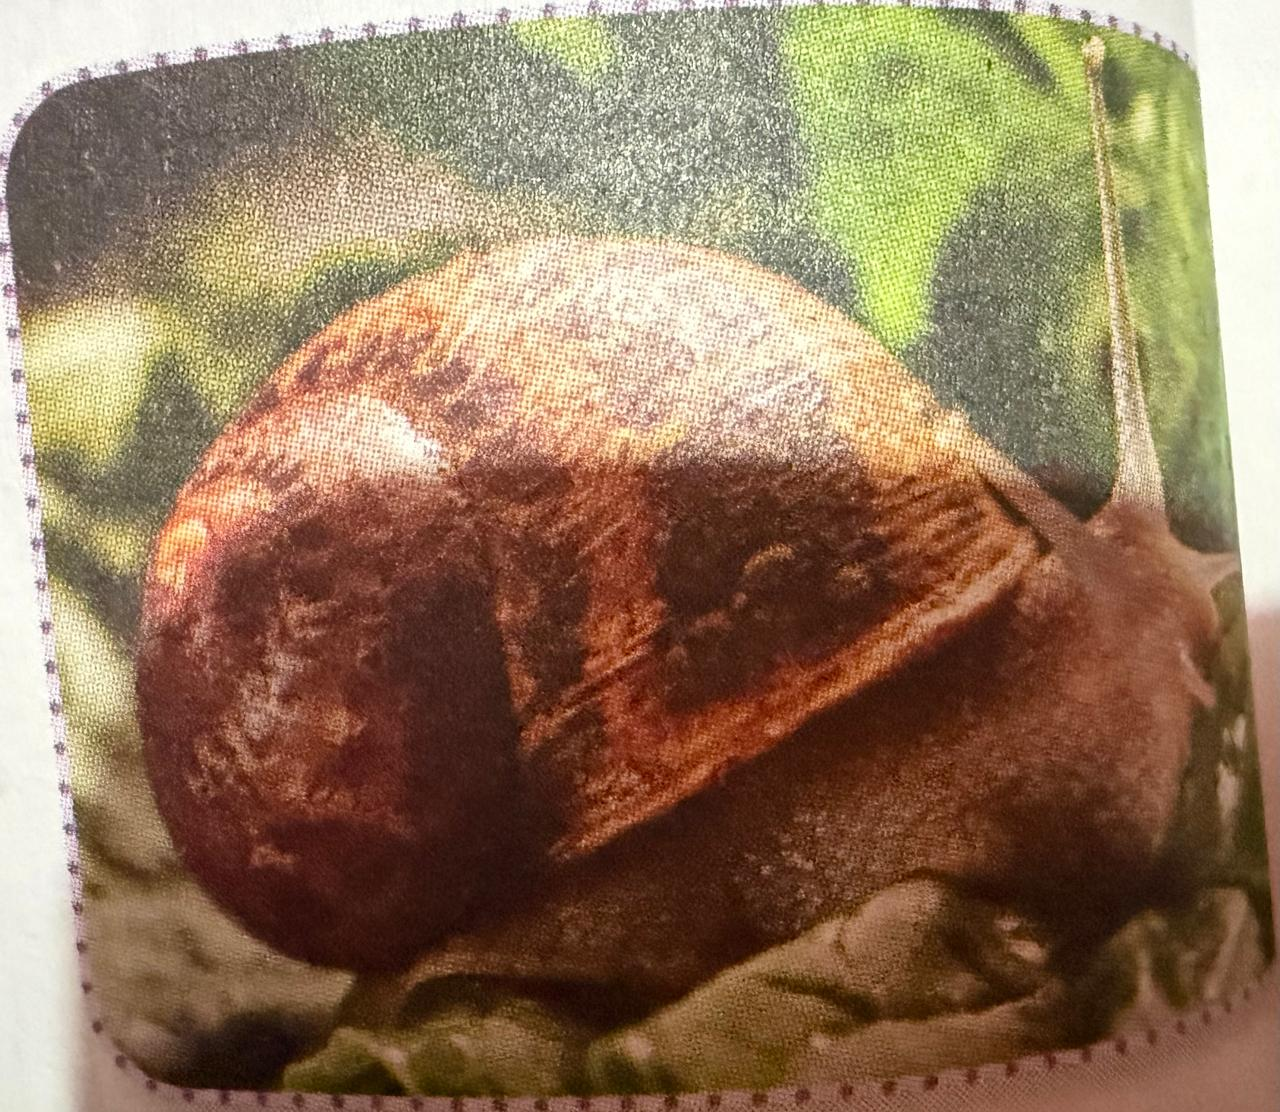
\includegraphics[width=0.5\linewidth]{../image/shell.jpeg}
    \caption{Caption}
    \label{fig:shell}
\end{figure}
\par\vspace{0.8in}
\subsection{\textcolor{orange}{Adaptations that Help to Breathe}}
All animals breathe in oxygen and breathe out in carbon dioxide. The body needs to be oxygen to burn food and release energy. Animals that live on land take in oxygen through air, whereas animals that live in water take in oxygen dissolved in water.\\
\par
Different animals have different organs that help them to breathe. Let us learn about the types of organs that animals use to breathe.\\
\par\vspace{0.2in}
\textbf{Lungs:} Lungs are the primary breathing organs in mammals, including humans. They are soft, spongy organs that help us breathe in oxygen from the air and release carbon dioxide.\\
\begin{figure}
    \centering
    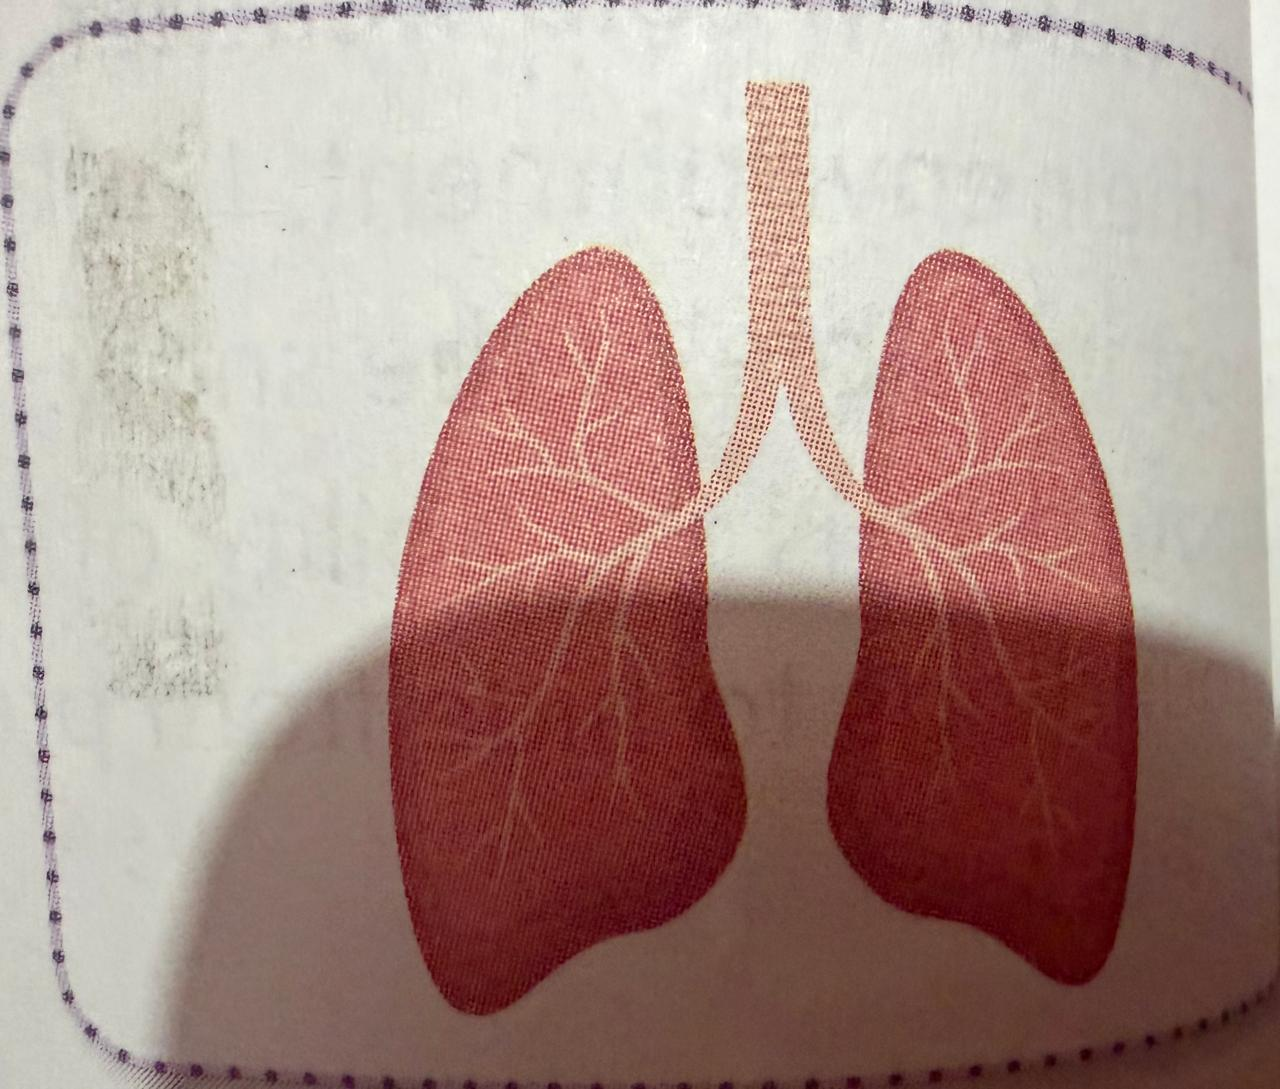
\includegraphics[width=0.5\linewidth]{../image/lungs.jpeg}
    \caption{Caption}
    \label{fig:lungs}
\end{figure}
\par
The lungs have a vast network of fine blood vessels. When air reaches the lungs, and exchange of gases takes place between the inhaled air and the blood. The oxygen is absorbed by the blood and carbon dioxide is given out.\\
\par
\textbf{Gills:} Gills are respiratory organs found in fish and some other aquatic animals like crabs, sharks and octopus. Gills take up oxygen from water when water passes over them, allowing these animals to breathe underwater.\\
\begin{figure}
    \centering
    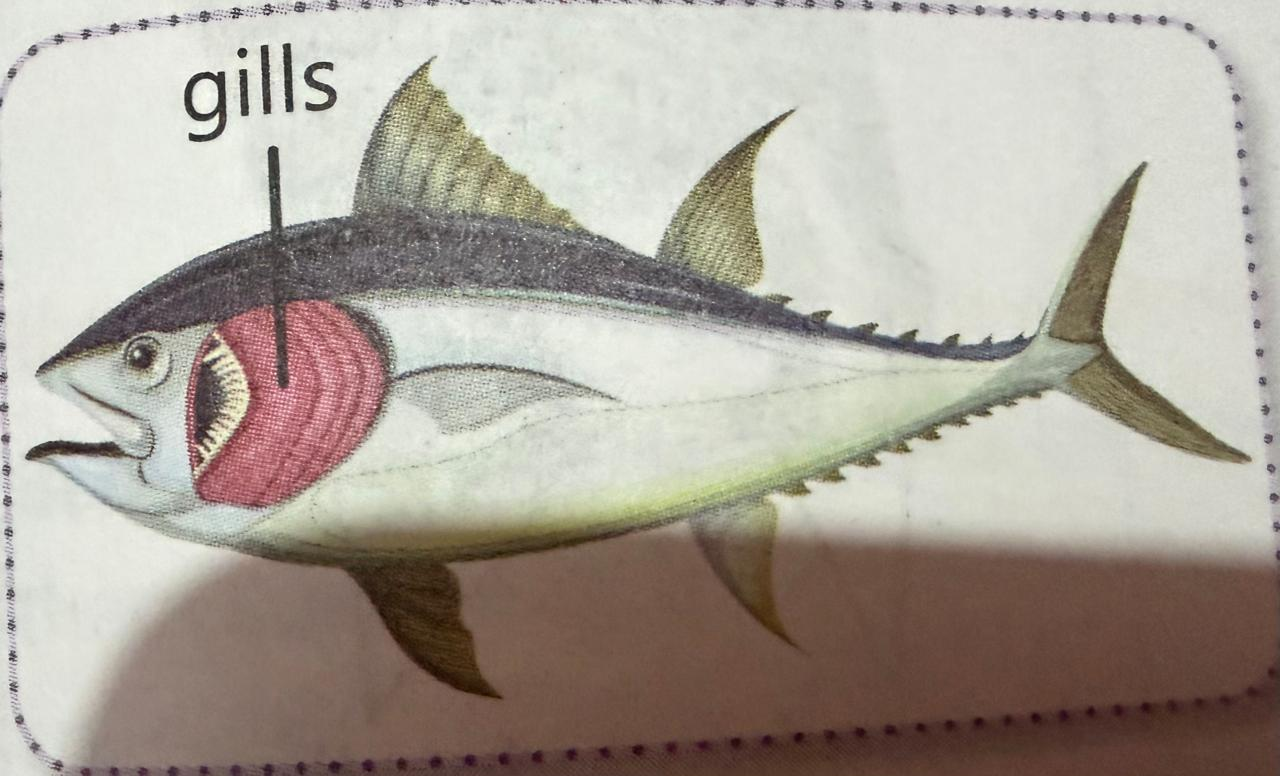
\includegraphics[width=0.5\linewidth]{../image/fish.jpeg}
    \caption{Caption}
    \label{fig:fish}
\end{figure}
\par
\textbf{Spiracles:} Spiracles are small openings found on the bodies of insects such as beetles and butterflies. They serve as the entry and exit points of air in an insect's respiratory system.\\
\begin{figure}
    \centering
    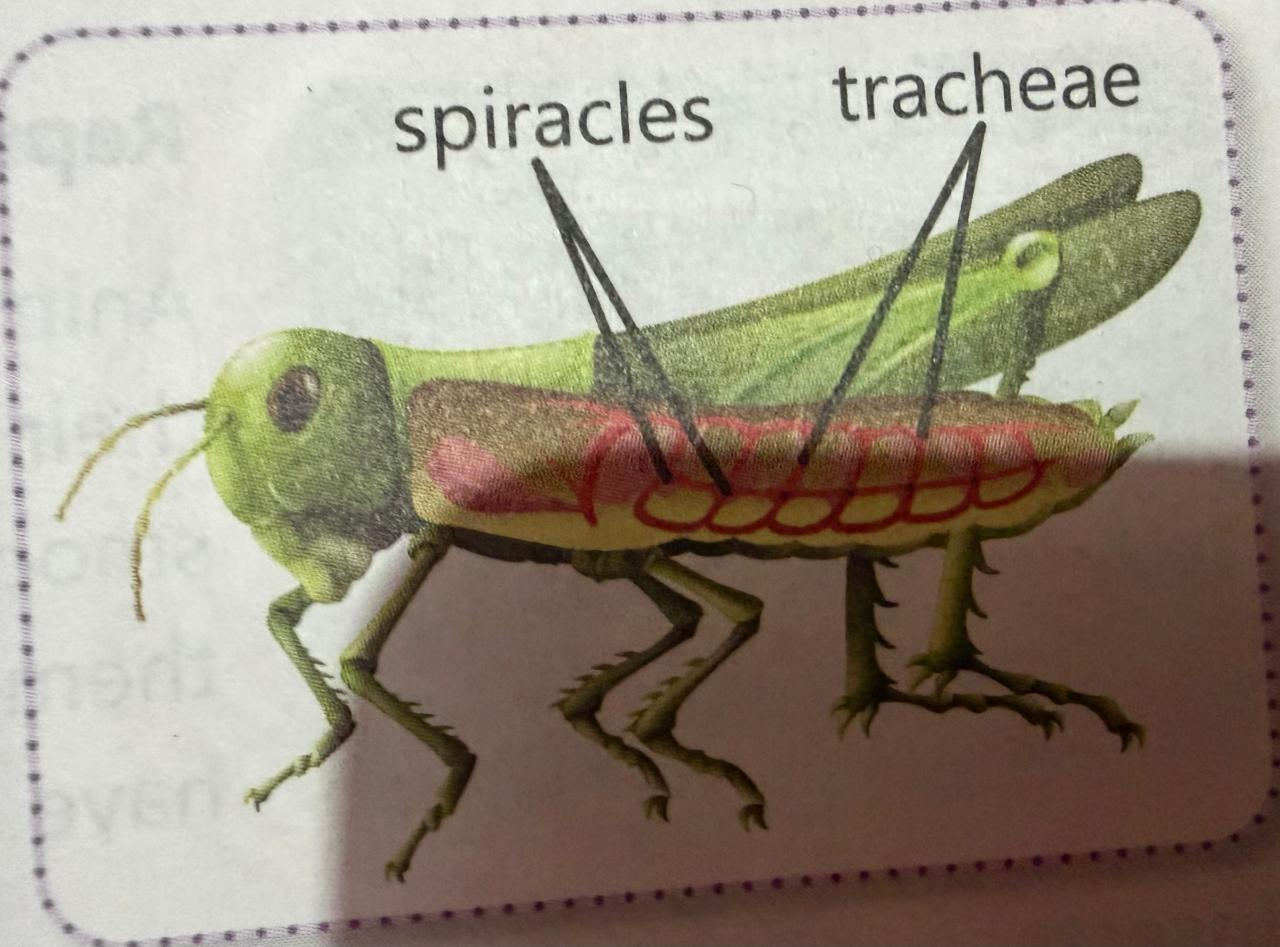
\includegraphics[width=0.5\linewidth]{../image/spiracles.jpeg}
    \caption{Caption}
    \label{fig:spiracles}
\end{figure}
\par
Air enters the spiracles and travels through a series of tiny tubes called \textbf{trachee}
\textbf{Moist skin:} Animals such as frogs and earthworms breathe through their moist skin.\\
Frogs breathe with the help of their moist skin when in water and with lungs when on land. Tadpoles live in water, and they breathe through gills.\\
\begin{figure}
    \centering
    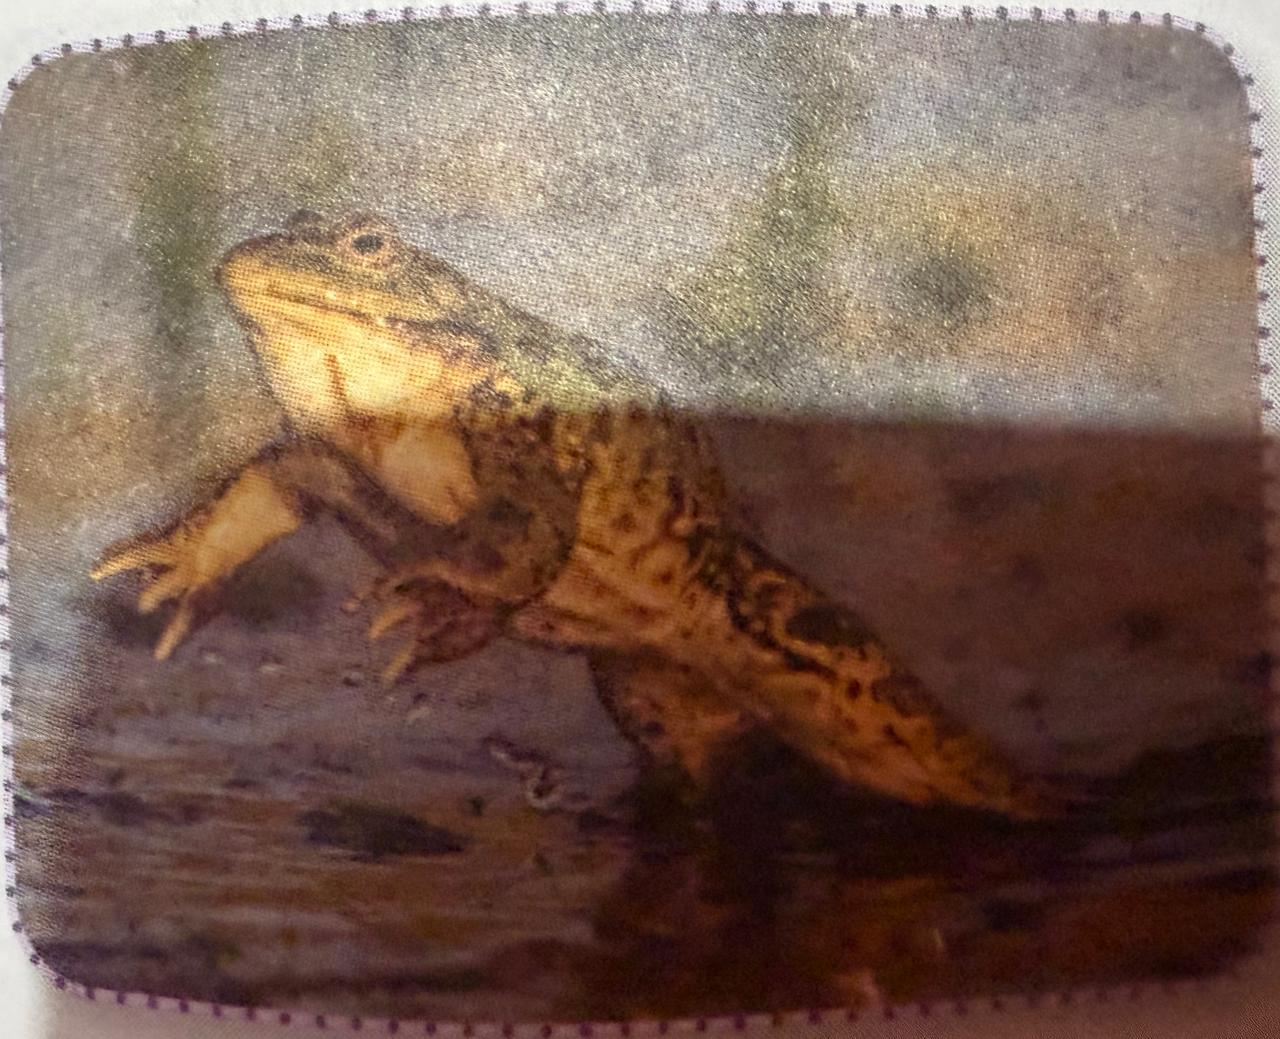
\includegraphics[width=0.5\linewidth]{../image/frog.jpeg}
    \caption{Caption}
    \label{fig:frog}
\end{figure}
\par
\textcolor{red}{I wonder} why humans cannot breathe underwater.
\subsection{\textcolor{orange}{Adaptations for Movements in Animals}}
Animals need to move in order to search for food, to escape danger, to adapt to the changing environment and to find suitable shelters. Different animals have different types of structures that helps in their movement. Let us learn about a few of them.
\subsection{\textbf{Mammals}}
Fore and hindlimbs are important body parts in mammals. \textbf{Forelimbs} are the front limbs and \textbf{hindlimbs} and the back limbs. These limbs help them in mammals. Forelimbs in many mammals help in grasping and holding things in addition to the movement. Hind limbs provide support and balance and also help in jumping and leaping.\\
\par
\begin{figure}
    \centering
    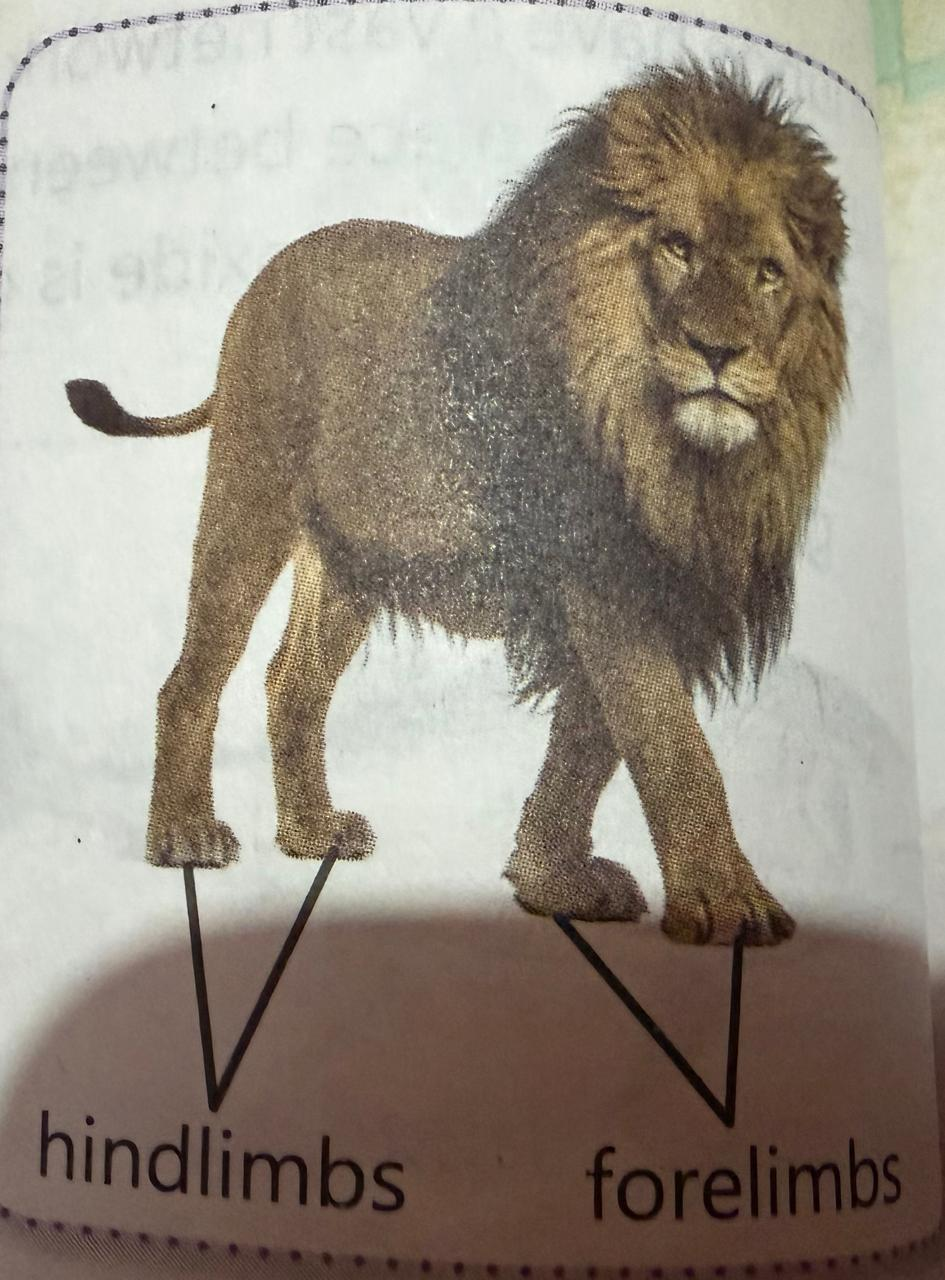
\includegraphics[width=0.5\linewidth]{../image/lion.jpeg}
    \caption{Caption}
    \label{fig:lion}
\end{figure}
In humans, hands from the forelimbs and legs from the hindlimbs.
\subsection{\textbf{Reptiles}}
Animals like lizards and crocodiles process scales underneath their bodies that help them crawl. These scales enable smooth movement along surfaces. Snakes \textcolor{red}{slither}. They propel themselves forward by slithering against the ground. They have a flexible backbone too.
\begin{figure}
    \centering
    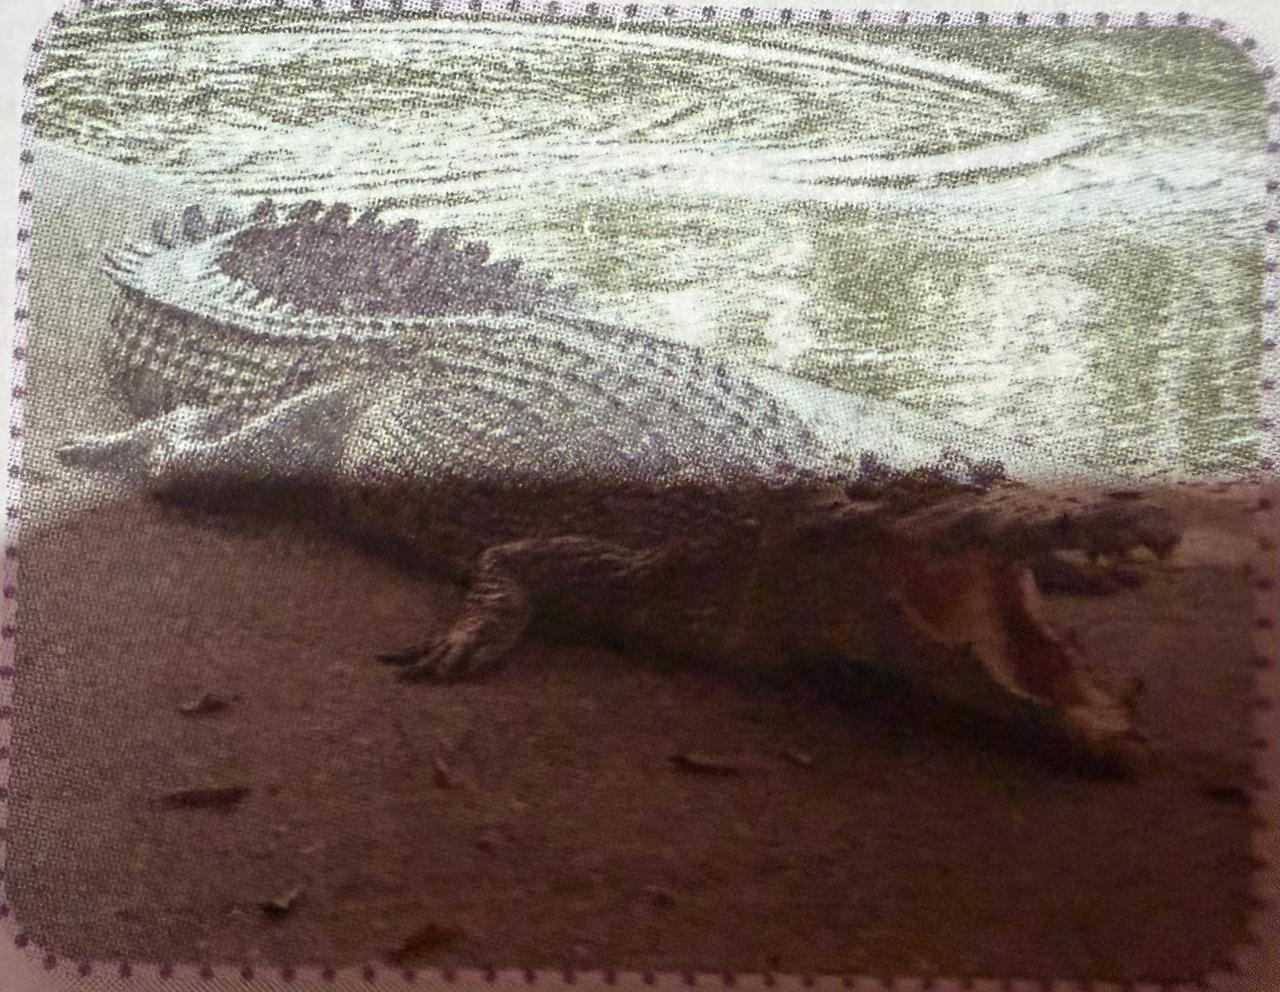
\includegraphics[width=0.5\linewidth]{../image/crocodile.jpeg}
    \caption{Caption}
    \label{fig:crcocodile}
\end{figure}
\subsection{\textbf{Insects}}
Most insects have three pairs of legs. Insects such as cockroaches and ants use legs to crawl. Some insects such as houseflies and butterflies have wings to fly.
\begin{figure}
    \centering
    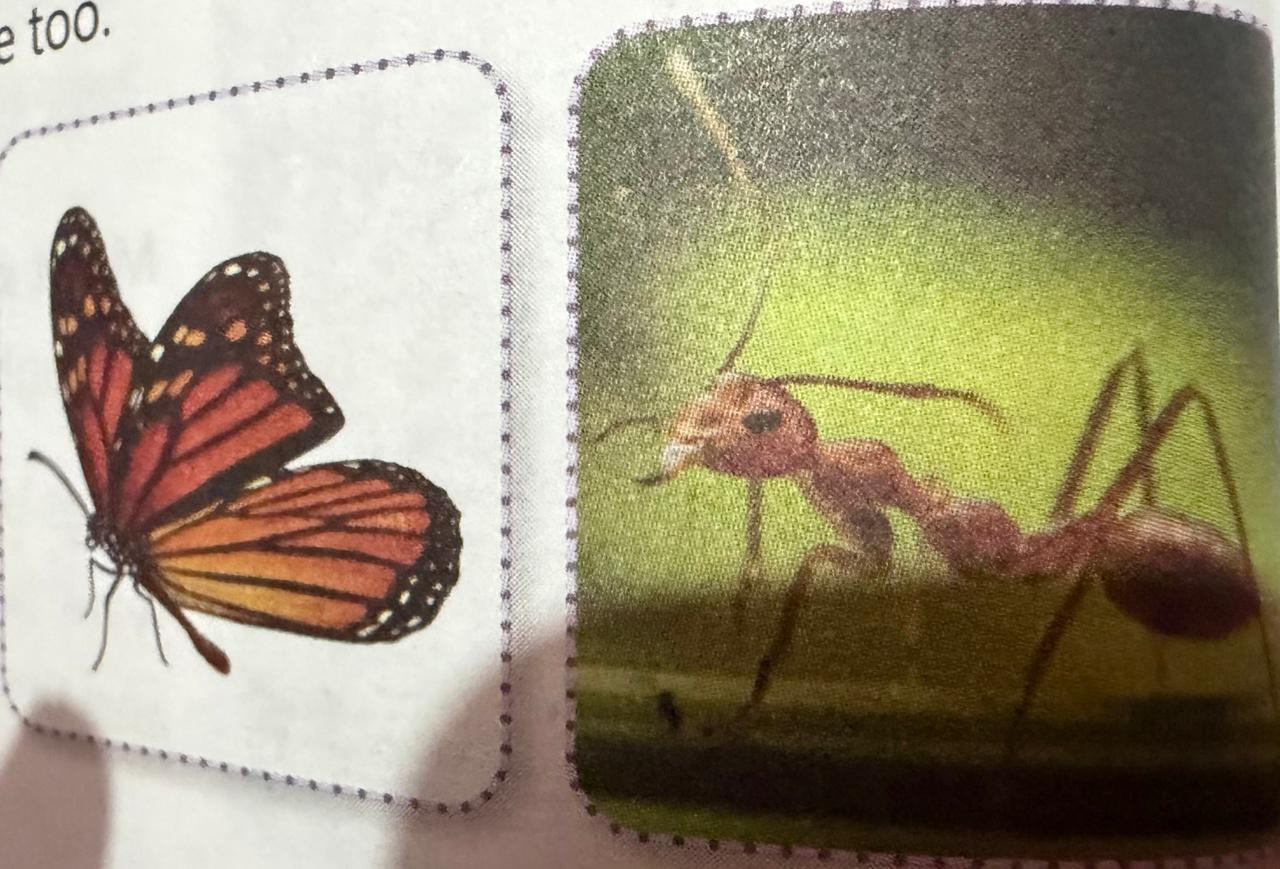
\includegraphics[width=0.5\linewidth]{../image/insects.jpeg}
    \caption{Caption}
    \label{fig:insect}
\end{figure}
\subsection{\textbf{Birds}}
Birds are capable of both flying and walking. Their bodies are \textcolor{red}{streamlined}. Their forelimbs are modified into wings, which are connected to their bones. Chest muscles help birds flap their wings. Wings consist of feathers help in altering the direction and smooth landing. Birds use their hindlimbs for activities such as walking, hopping and perching. \\
\par
These are some flightless birds too. Examples of flightless birds include ostriches, emus, rheas and penguins.
\begin{figure}
    \centering
    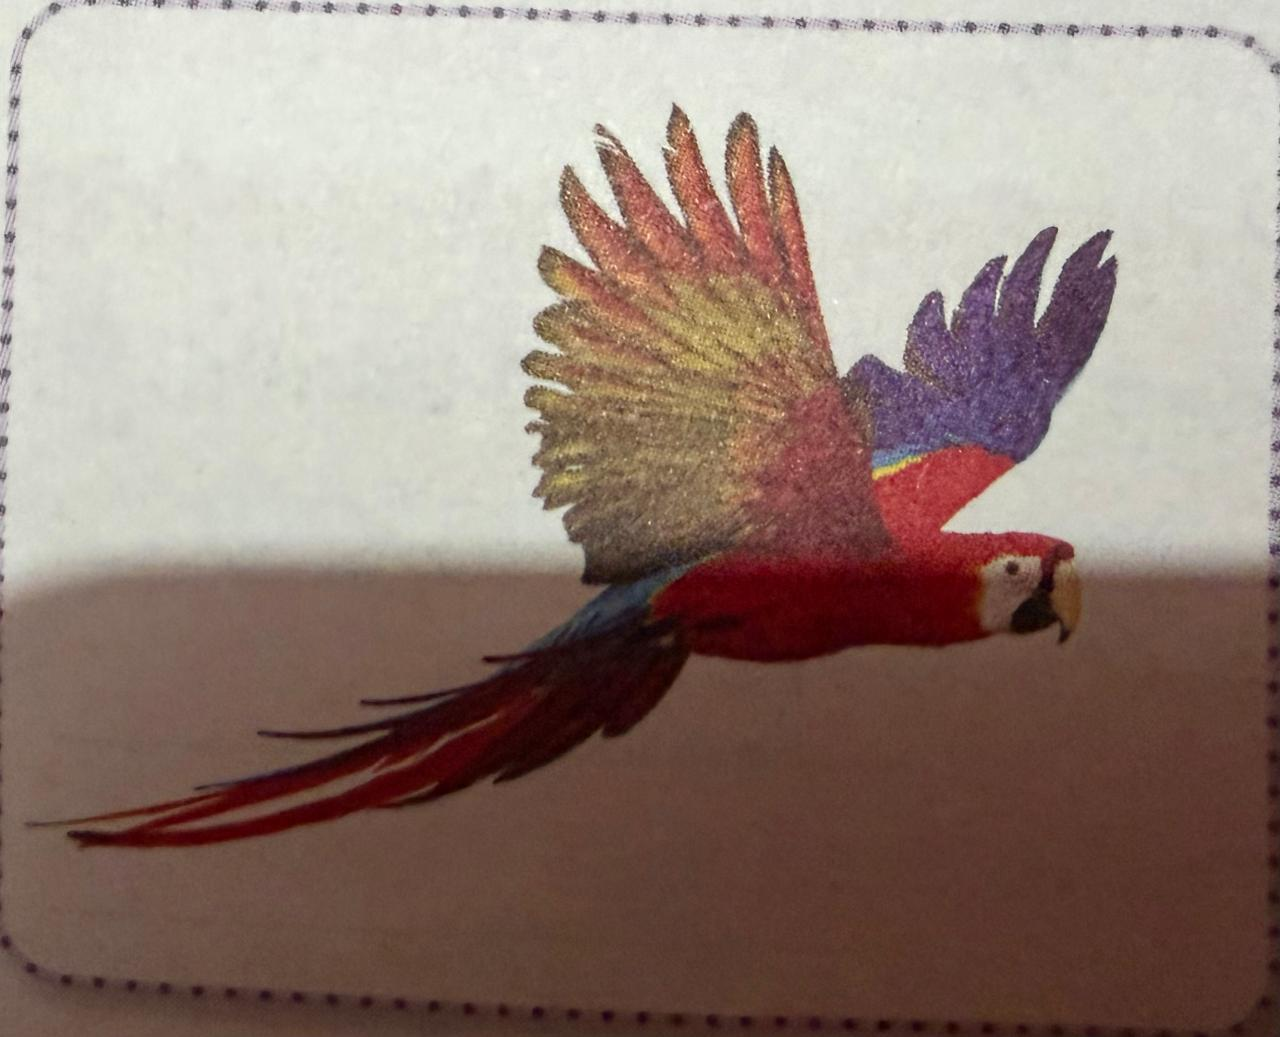
\includegraphics[width=0.5\linewidth]{../image/bird.jpeg}
    \caption{Caption}
    \label{fig:my-bird}
\end{figure}
\begin{figure}
    \centering
    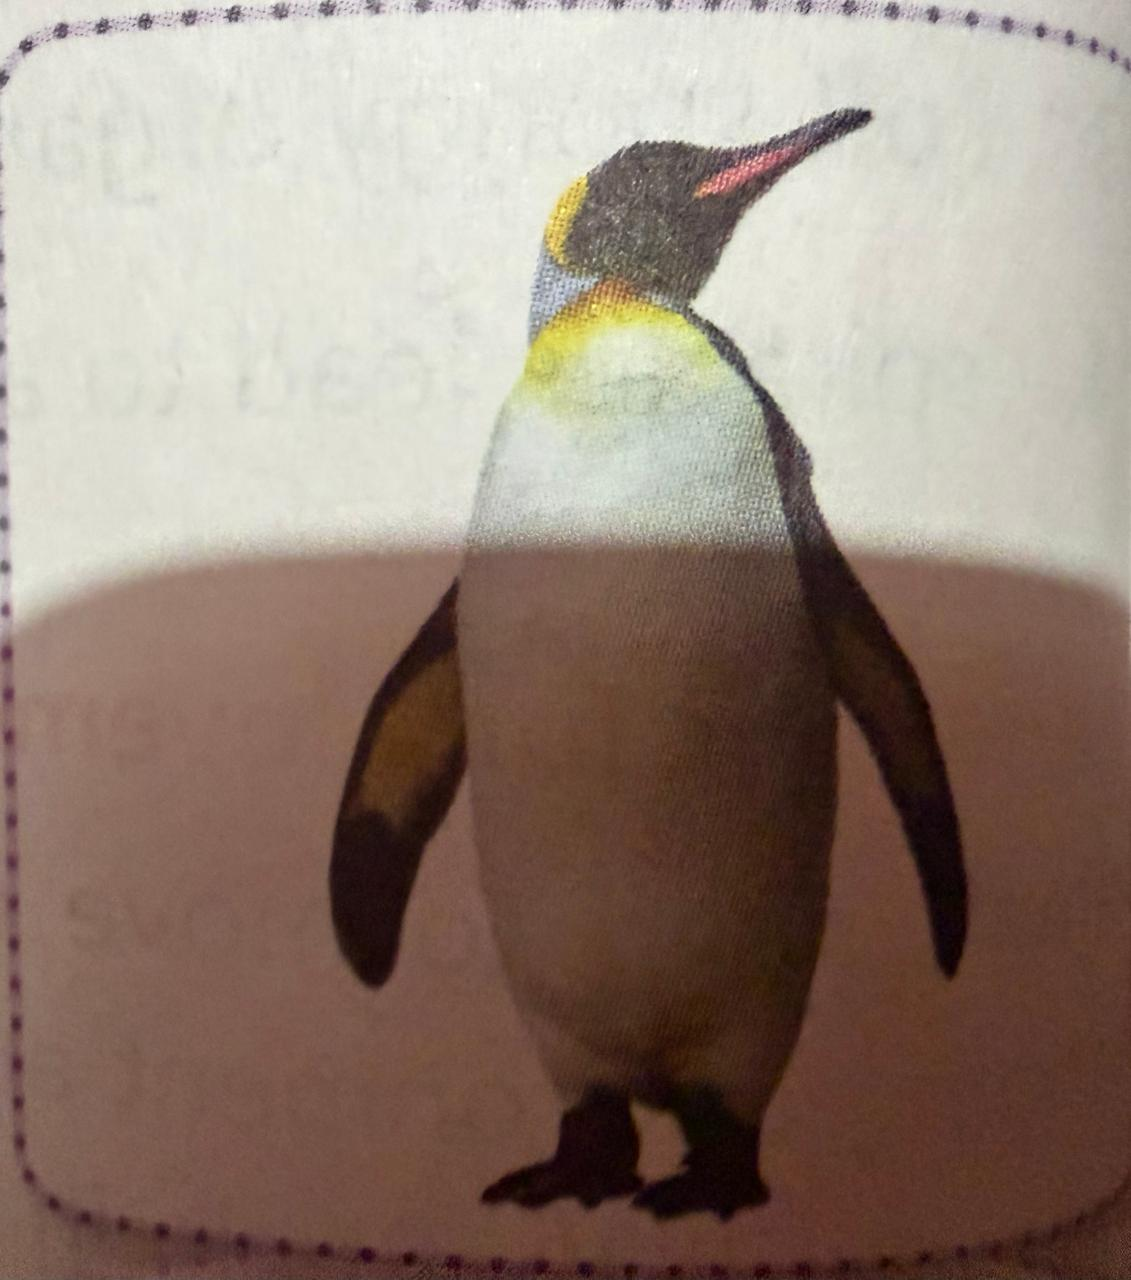
\includegraphics[width=0.5\linewidth]{../image/penguin.jpeg}
    \caption{Caption}
    \label{fig:penguine}
\end{figure}
\subsection{\textcolor{orange}{Behavioural Adaptations in Animals}}
\textbf{Behavioural adaptations} are specific actions or behaviours that animals develop to help them survive in their environments. Here are some examples of behavioural adaptations in animals.
\subsection{\textbf{Migration}}
Some birds travel long distances during different seasons. This is called \textbf{migration.} They do this to find better plants to reproduce. Migration helps them avoid harsh wheather conditions are find safer environments.\\
\par
Siberian white cranes migrate to India during winters from Western Siberia.\begin{figure}
    \centering
    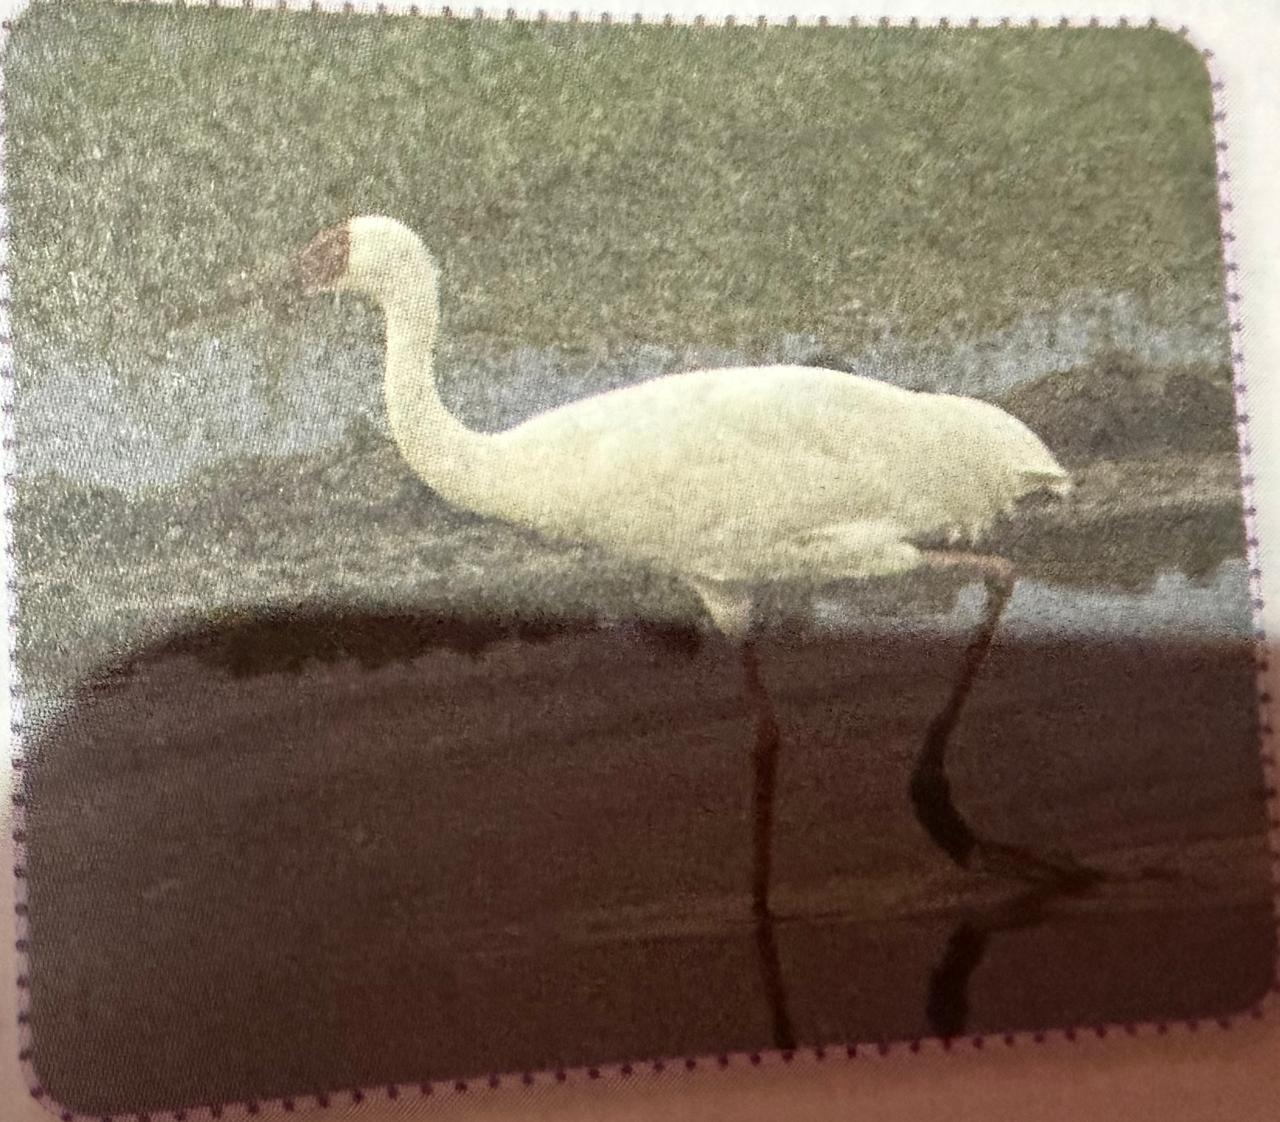
\includegraphics[width=0.5\linewidth]{../image/Swan.jpeg}
    \caption{Caption}
    \label{fig:swan}
\end{figure}
\subsection{\textbf{Hibernation}}
Certain animals, such as bears and bats, go into a deep sleep called \textbf{hibernation} during the winter months when the food is scare. They do this to conserve their energy. Hibernation allows them to survive periods of extreme winters and food scarcity.
\subsection{\textbf{Group Behaviour in Animals}}
Many animals live and work together in groups or communities. Ants live in colonies, wolves in packs and zebras in herds. Living in groups helps animals protect themselves from predators, find food more efficiently and raise their young ones collectively.
\begin{figure}
    \centering
    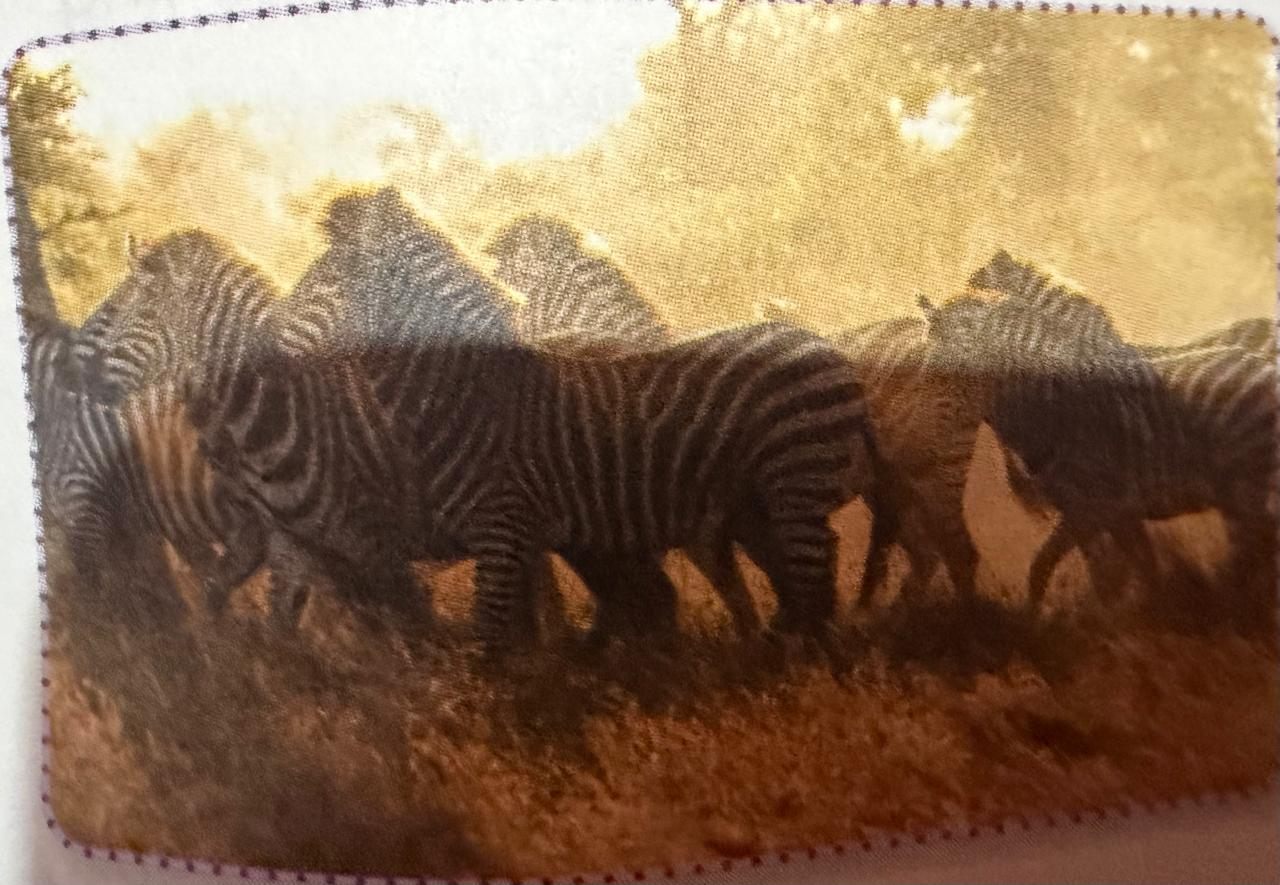
\includegraphics[width=0.5\linewidth]{../image/Zebras.jpeg}
    \caption{Caption}
    \label{fig:zebras}
\end{figure}
\section{\textcolor{red}{Endangered Animals}}
\textbf{Endangered animals} are animals that are at the risk of disappearing from the earth.\\
\par
There are different reasons why animals become endangered, such as habitat destruction, pollution, climate change and \textcolor{red}{poaching}.\\
\par
Among the endangered animals are the black rhinoceros, mountain gorilla and apur leopard.\begin{figure}
    \centering
    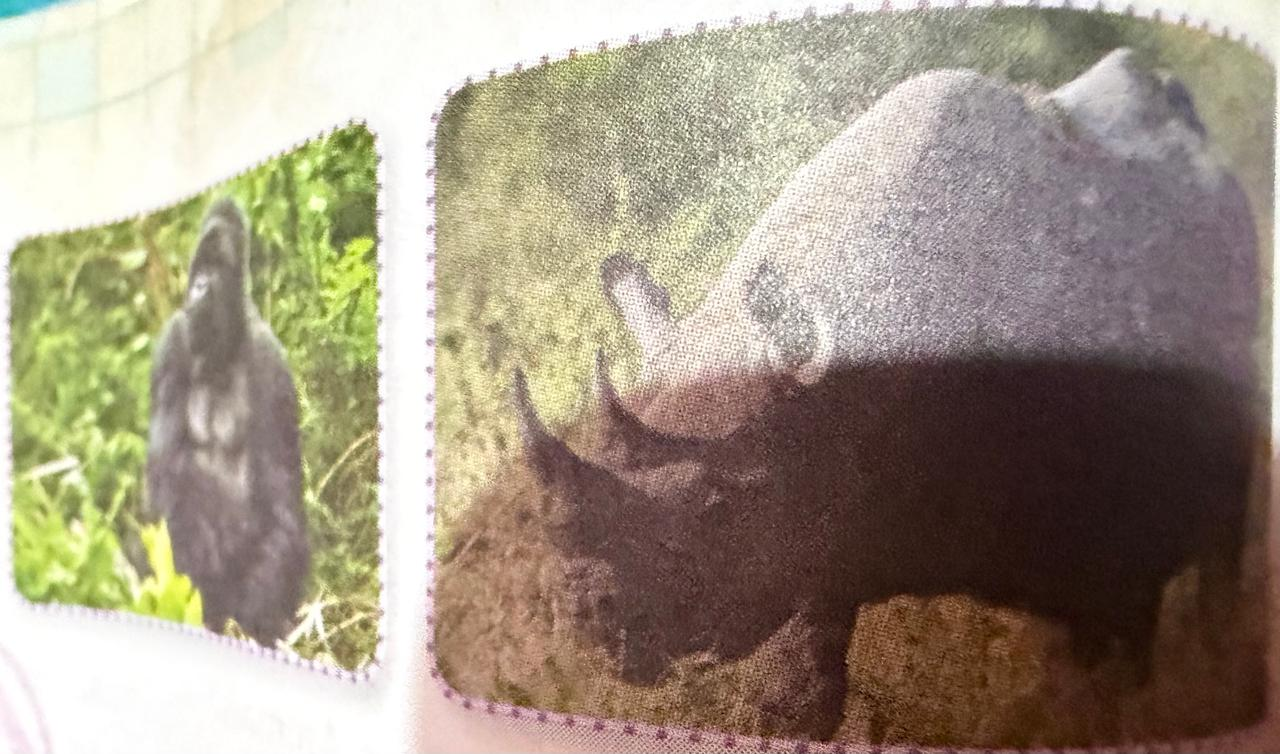
\includegraphics[width=0.5\linewidth]{../image/endangered_animals.jpeg}
    \caption{Caption}
    \label{fig:eanimal}
\end{figure}
\begin{itemize}
    \item \textbf{A habitat} is the natural home or an animal where it lives, grows, eats and reproduces.\\
    \item \textbf{Adaptations} are the changes in the bodies or behaviours of animals that help them survive better in their environments.\\
    \item Different types of body coverings like fur, feathers, scales and shells help animals protect themselves from various environmental conditions.\\
    \item Animals have different adaptations that help them breathe - lungs, gills, spiracles, moist skin, etc.
    \item Animals have different adaptations that help in their movement - forelimbs, hind limbs, wings, scales, streamlined bodies, etc.
    \item Hibernation, migration and group behaviour are some of the behavioural adaptations that animals show.
\end{itemize}
